\chapter{Introduction}
\label{chap:introduction}
\pagenumbering{arabic}% Arabic page numbers (and reset to 1)
In this chapter, the topic of this dissertation is first positioned in the research area and its objectives are developed. Following, a more specific definition of the topic will be given. Subsequently, the research objective and hypothesis will be presented.
\section{Background}
Dead zones (DZ) are regions separated from the main channel and its principal characteristic is the net flux close to zero in the main stream direction. They can be formed by any structure that creates an irregularity withing the water body morphology, examples of structures are: groyne fields, lateral cavities, vanes, harbours and sidearms. The shared characteristic of these zones is its closeness, except for a single interface, the volume is completely dissociated from the main channel. This implies that the study of this interface is essential to understand all the exchange processes between the DZ and the main channel. Normally placed in shallow waters, the transport inside the DZ is regarded as a two-dimensional motion, except for the interface between the unaltered channel (main channel) and the DZ where complex three-dimensional motion occurs \cite{xiang2020}. The typical path in the interface follows the order where the fluid penetrates the DZ near the bottom of the channel and exits primarily in the top layer of the flow, also it enters approximately via the downstream portion and exits in the upstream of the DZ \cite{weitbrecht2004,xiang2020}. As one of the main metrics in mass transport in DZ is the mean retention time, it is implied that this kind of flow can be considered as a transient storage volume.

The transient storage of mass inside the DZ has been known to provide refuge to aquatic communities as they seek shelter in slower-moving flows in the surface stream or the hyporheic zone \cite{jackson2013}. According to the same author, the benefits of this storage extends to water quality improvement as the solutes residence times increases further increasing the interaction of nutrient-rich surface waters with biogeochemically-reactive sediments. For instance, \textcite{SchwartzKozerski2003} detected in their sample larger amounts of element contents with sedimentary origin than from geogenic sources, the increase in mass settled to the riverbed can become favourable to vegetation growth (Figure \ref{fig:satelliteImage}). The drag created by the presence of vegetation changes the flow and consequently the mass exchange rates, which increases the uncertainty of volumes captured within the seasons.

\begin{figure}[!ht]
\centering
\begin{subfigure}{0.49\textwidth}
  \centering
  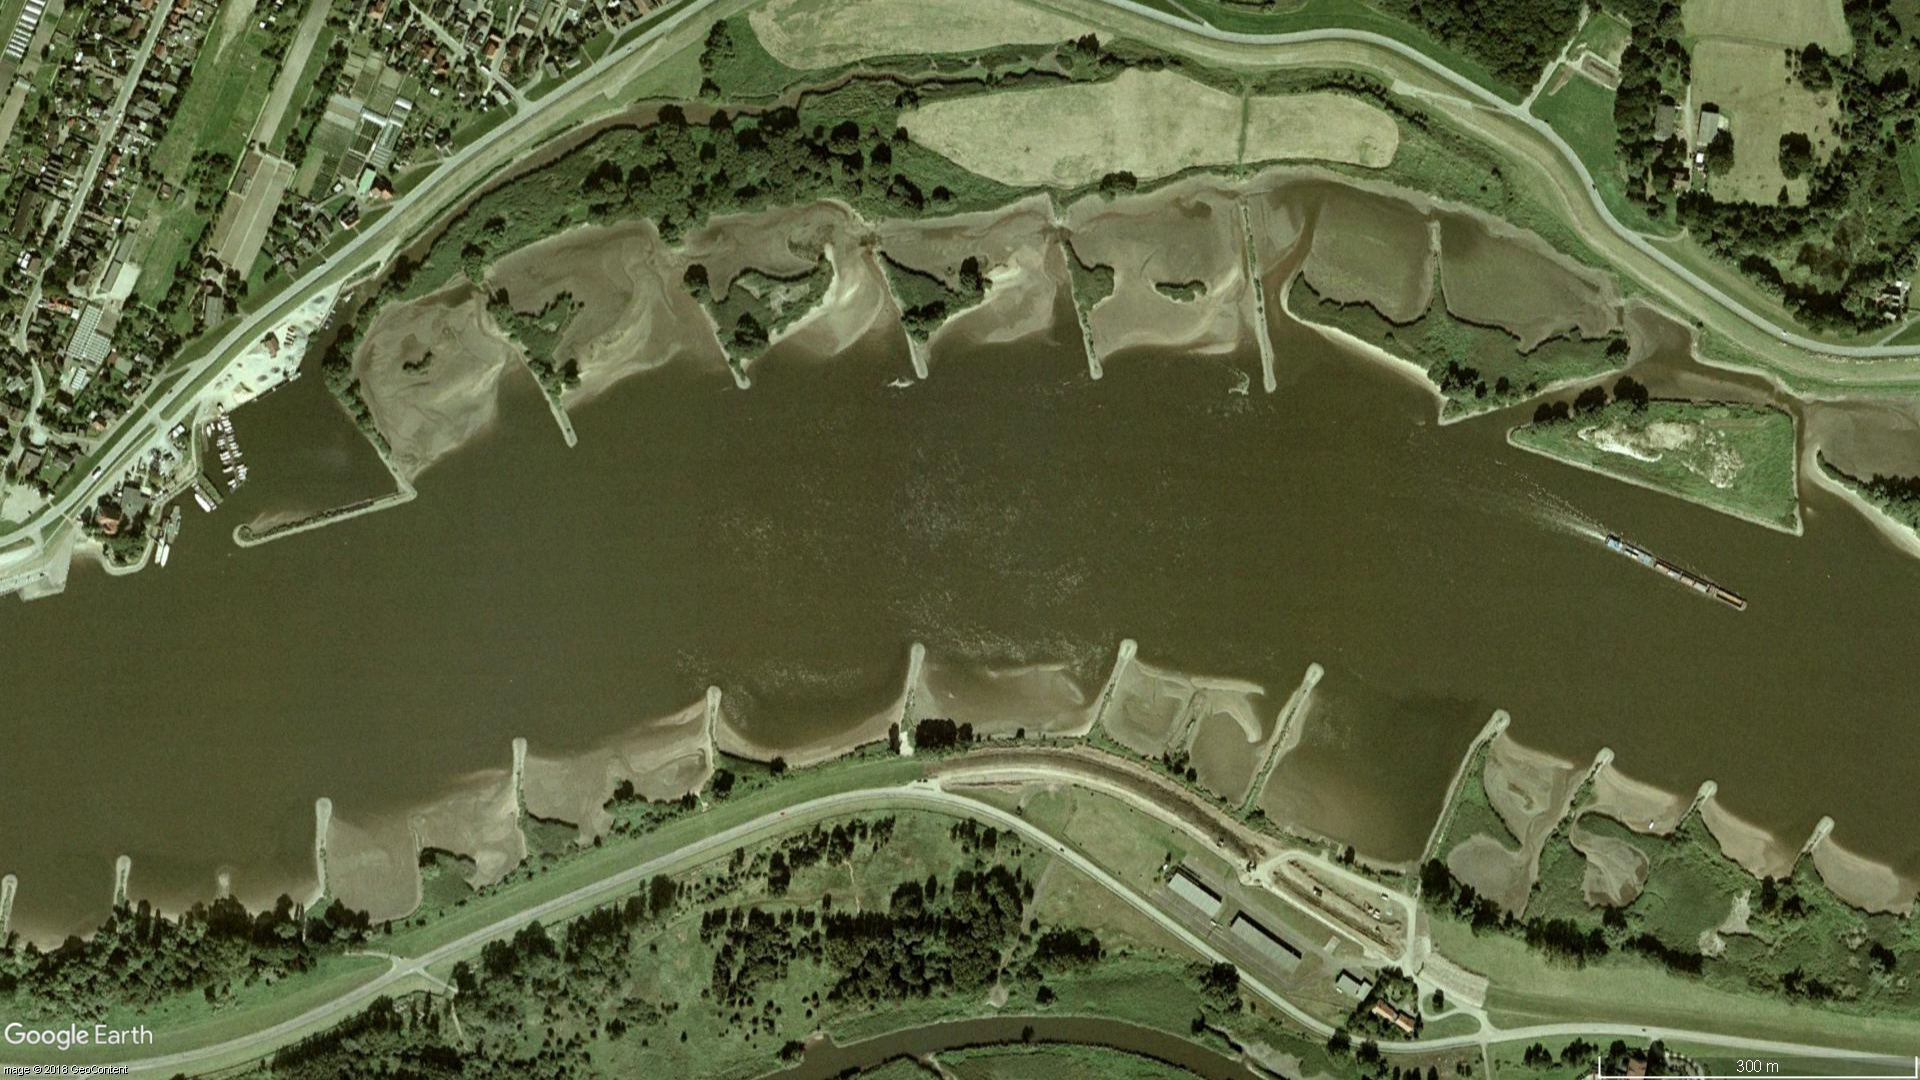
\includegraphics[width=0.9\linewidth]{../images/introduction/sat2000.jpg}
  \caption{2000}
  \label{fig:sat2000}
\end{subfigure}%
\begin{subfigure}{.49\textwidth}
  \centering
  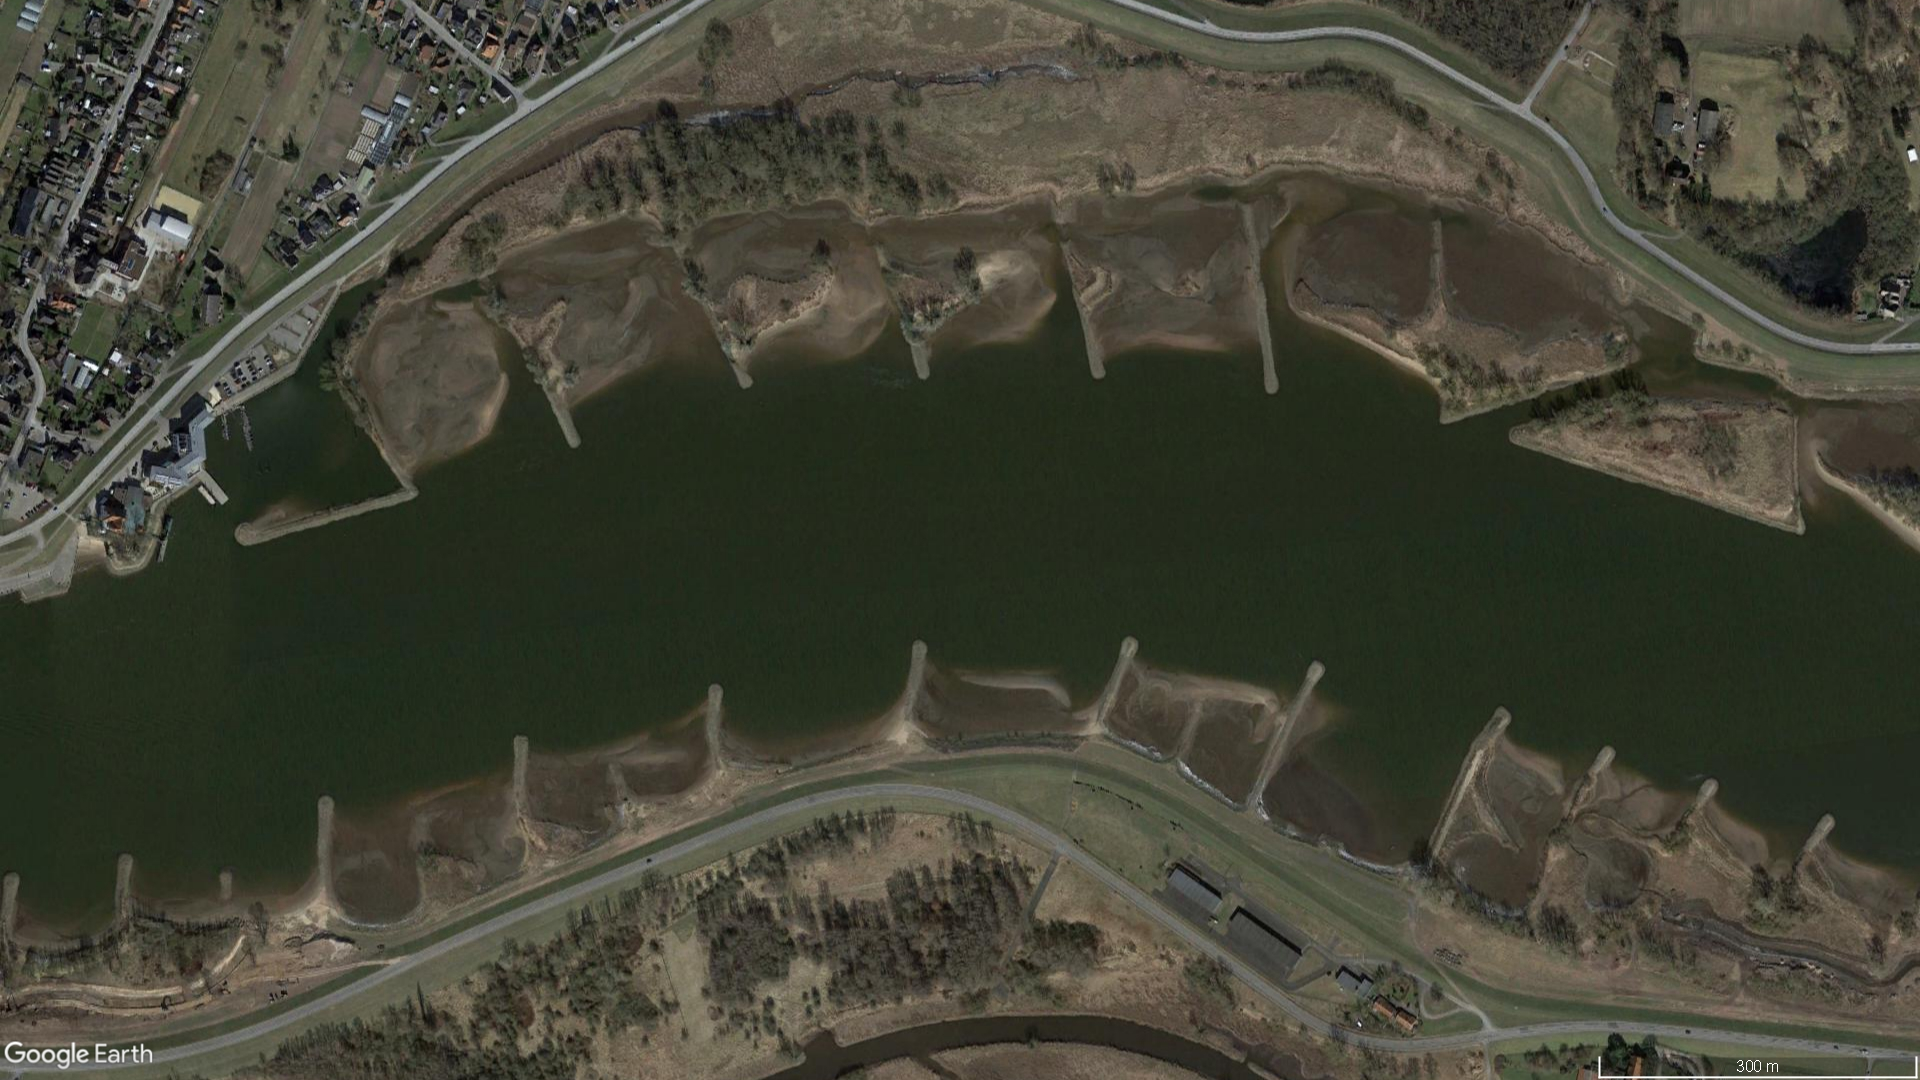
\includegraphics[width=0.9\linewidth]{../images/introduction/sat2018.jpg}
  \caption{2018}
  \label{fig:sat2018}
\end{subfigure}
\caption{Groyne Fields 53\degree23'54.32" N,  10\degree11'51.08" E, elevation 1.90 km. Terrain layer, viewed 29 August 2019. <http://www.google.com/earth/index.html>}
\label{fig:satelliteImage}
\end{figure}

Lateral cavities are an important type of DZ in rivers, these regions can be considered an extension from the cross-sectional profile of the water body. The importance of this element is due (1) the enhancement in biodiversity \cite{ribi2014,harvey2016}, (2) the function as a macro-roughness at the river banks, mitigating erosion \cite{juez2018} and (3) act as a transient storage zone \cite{jackson2013,drost2014,jackson2015}.The principal characteristic of the flow, in an emergent scenario, is the presence of gyres. These vortexes origin from the dissipation of moment that occurs in the interface layer between the DZ and the main channel. The shearing and flow separation at the leading edge form a mixing layer that extends until the downstream portion of the lateral cavity \cite{uijttewaal2005,jackson2013}. The shape and quantity of circulations inside the cavity are determined by a geometric aspect between the width (normal to the flow, \textit{W}) and length (parallel to the flow, \textit{L}) of the cavity. The aspect ratio \textit{W/L} divides the flow in three configurations: (a) $W/L<0.5$ results in multiple circulations parallel to the main stream; (b) $0.5<W/L<1.5$ results in a single circulation; and (c) $W/L>1.5$ results in multiple gyres transversal to the main stream \cite{weitbrecht2001,jackson2013,sukhodolov2014}(Figure \ref{fig:lCavitySchema}).

\begin{figure}[!ht]
\centering
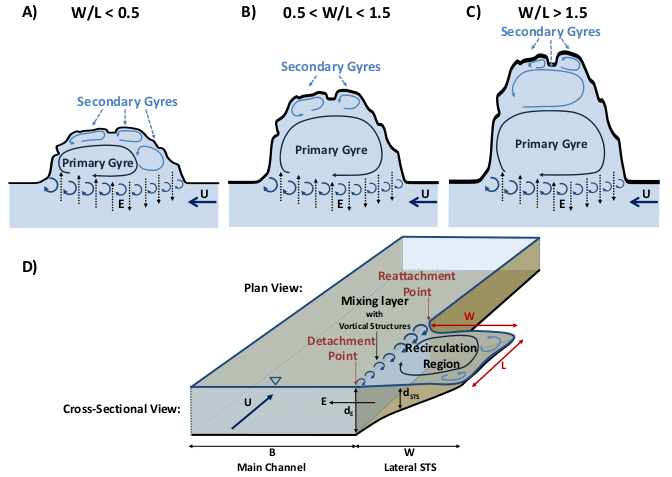
\includegraphics[width=0.9\linewidth]{../images/introduction/lateralCavitySchema.png}
\caption{Schema on the flow patterns of emergent lateral cavities \cite{jackson2013}}
\label{fig:lCavitySchema}
\end{figure}

The number of circulations in the system impacts on the mass exchange between the DZ and the main channel. As the mass decay inside the DZ follows a quick exponential decay in the early stages the rates get slower as the primary gyre transfers its mass out, in multiple gyres systems \cite{jackson2012}. After the main gyre transfers its mass, a slower exchange takes place between the second circulation into the primary one, since the velocity magnitudes in the secondary gyre are slower than the primary one. Henceforth, the mean residence time inside the DZ depends on the primary gyre residence time (early decay) and the secondary gyre volume (late decay) \cite{jackson2013}.

Another typical DZ structure is the groyne field, it consists of a series of lateral cavities inside the channel course. This DZ is created by transversal structures placed on the river bank, named groynes these structures diverges the flow creating a rotational field. The characteristics of the flow are somewhat similar to lateral cavities, especially on the geometric aspect ratio that predicts the number of circulations \cite{weitbrecht2004,uijttewaal2005,xiang2020}. Although an important difference is in the stabilisation of the mixing layer, this region growths until the fourth-sixth rank until it reaches a developed state (Figure \ref{fig:groyneStabilisation}), in other words, once it stabilises the width of the interface the flow becomes \textit{permanent} \cite{weitbrecht2004, mcCoy2008, xiang2020}.

\begin{figure}[!ht]
\centering
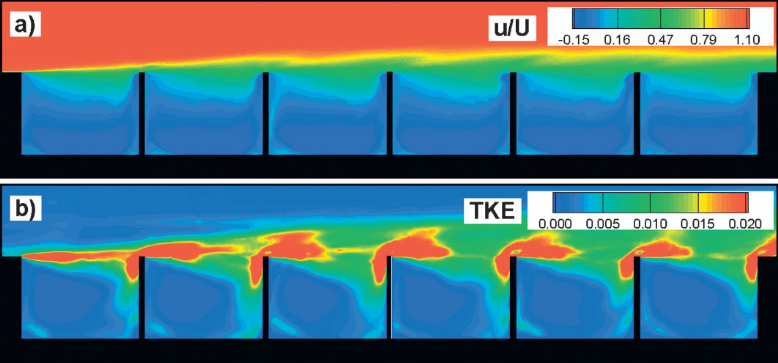
\includegraphics[width=0.9\linewidth]{../images/introduction/groyneStabilisation.png}
\caption{Time averaged quantities at $z/h=0.95$: a) streamwise velocity and b) TKE \cite{mcCoy2008}}
\label{fig:groyneStabilisation}
\end{figure}

\section{Methods of estimating the mass exchange }
\subsection{Interface velocity}
The mass exchange between DZ was vastly studied in the field, experimental and numerical studies. As the effects of the exchange occur in a confined volume, \textcite{weitbrecht2001} proposed a model to account the exchanges in the interface between the zones. This method only requires geometrical parameters and the mean transversal velocity in the interface surface, as shown in the mass exchange coefficient ($k$) of equation \ref{eqn:kvelocity}.
\begin{equation}
k=\frac{\overline{E}LH_E}{L WH_{DZ}}=\frac{1}{T_D}
\label{eqn:kvelocity}
\end{equation}
where, $H_E$ (m) and $H_{DZ}$ (m) are the water depth in the interface and in the DZ respectively, $\overline{E}$ (m/s) is the average transversal velocity in the interface, $L$ (m) is the length of the cavity, $W$ (m) is the width of the cavity and $T_D$ (s) is the mean residence time. The calculation of $\overline{E}$ depends on the surface averaging of the time averaged velocities and is given by the following equation:
\begin{equation}
E = \frac{1}{2A}\int_{A}^{}\left | v \right |dA
\label{eqn:exchangeVel}
 \end{equation}
 where $A$ (m$^2$) is the area of the interface and $v$ (m/s) is the transversal element of time averaged velocity vector.

Despite this planar method give a good approximation on the exchange velocity the effect of mass diffusivity is neglected, this further implies that systems slower circulations will have a larger impact of the estimated $k$. One can assume that this methodology works for conventional DZ, although it must be taken carefully for vegetated systems as the mixing layer alone may influence the result of $k$.
\subsection{Tracer fields}
Another approach on the mass exchange is through tracer experiments, that can be divided into washout and pulse procedures.  This method treats the mass exchange in tridimensionally as all the flow variables are considered. This approach gives a better understanding of the exchange in all conditions as it provides more information, for instance, the tracer methodology allows one to study the behaviour of mass in local regions of the volume or as a global volume. \textcite{weitbrecht2004} conducted a series of experiments on groynes both using the equation \ref{eqn:kvelocity} and a first-order mass decay (equation \ref{eqn:massDecay}). The results of both methods were compared and the velocity and tracer method agreed only in 12.5\% of the cases. From his data, it appears that single circulation systems tend to have the $k_{vel} < k_{tracer}$, while the opposite occurs in multiple gyres systems. A possible reason for this phenomena is that the second slope provided by the secondary circulation retards the mass exchange accounted by the tracer, as the velocity field only considers the interface this effect is not captured and thus the mass exchange is slightly higher.
\begin{equation}
C(t)=C_0e^{-t/T_D}
\label{eqn:massDecay}
\end{equation}
where $C_0$ is the initial tracer concentration, $t$ (s) is time and $T_D$ (s) is the mean residence time, variable that is fitted into the equation using the volume averaged tracer concentration on available times. The mass exchange would then be calculated as:
\begin{equation}
k=\frac{W}{T_D U}
\label{eqn:ktracer}
\end{equation}
where $U$ (m/s) is the mean velocity in the main channel.

The advantage of this method is data richness that it provides, especially in numerical experiments. Some additional studies can be done to analyse other phenomena associated to mass, for instance, one can use a decay to estimate the amount of mass that is treated by plants or a settling velocity to preview sedimentation in the DZ. The only side effect of this method is the increased complexity to perform these experiments, be the difficulty in controlling the volume of water in the field or the calibration of the turbulent Schmidt number ($S_{ct}$) in numerical studies. 
\section{Vegetation Impacts}
The influence of vegetation in the mass exchange in lateral cavities was first studied in \textcite{xiang2019}, that will be discussed in this paragraph. In this paper, a single lateral cavity was studied with a varied vegetation density. The vegetation was represented as solid cylinders inside the cavity volume. The cavity was emergent with a single circulation, due to its $W/L=0.6$. The vegetation density ($a$) ranged from 0 to $6.27\permil$ and as it increased more drag was introduced into the flow resulting in a slower circulation inside the volume. The turbulent kinetic energy in the DZ gradually due to the blockage that impeded high energy vortexes from entering the volume. The effect on mass exchange occurred in two phases: first, there was a decay in the mean residence time due to the plant induced Karman vortex street and the plant blockage since the mixing rate from the vortex is greater than the blockage; in a second phase $a>3.96\permil$ the blockage was higher than the mixing what increases of mean residence time (Figure \ref{fig:xiang2019fig12}).
\begin{figure}[!ht]
\centering
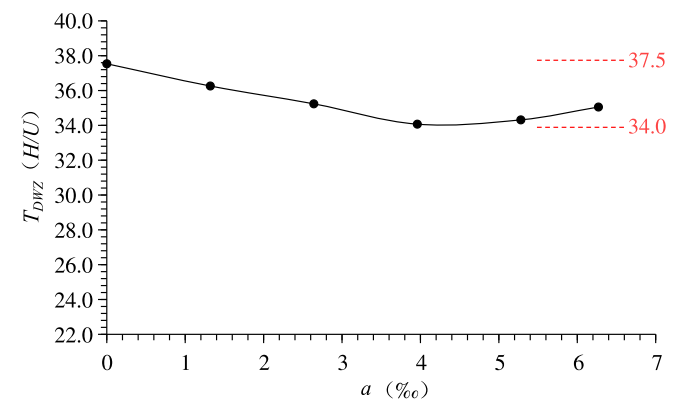
\includegraphics[width=0.8\linewidth]{../images/introduction/xiang2019fig12.png}
\caption{The variation of mean residence time ($T_{DWZ}$) with the increase of vegetation density ($a$) \cite{xiang2019}.}
\label{fig:xiang2019fig12}
\end{figure}

Despite the comprehensive density range, some aspects more related to field measures were left. For instance, in a vegetated groyne field, the vegetation levels were up to $15.7\permil$ \cite{sukhodolov2017}. A larger vegetation density range may contain other phenomena that could not appear in the previous study from \textcite{xiang2019}. This hypothesis indicates that studying the variation of density until the vegetation resistance blocks the flow would cover all the possible ranges and thereby phenomena associated with this flow.

The study with vegetated cavities still could not identify a threshold for vegetation to be considered "dense" or "sparse" in cavities, and its understanding will allow researchers to identify flow modifications in the cavity (e.g., the suppression of recirculation gyres, the complete suppression of flow, the exchange coefficient asymptote, etc.).  For emergent vegetation patches in an open channel, \textcite{chen2012} characterised them as being “dense” or “sparse” according to flow blockage thresholds, in which the flow properties near the patch (e.g., flow adjustment length and the velocity exiting the patch) were distinct above and below the threshold. A similar approach can be done for vegetated cavities. 
\section{Objective and Research Questions}
Given the importance of the exchanges in lateral cavities in natural rivers, the objective of this study is:

\textit{To describe the influence of vegetation in the mass exchange between a lateral cavity and the undisturbed section of the flow.}

Important considerations in this study area:
\begin{itemize}[noitemsep,topsep=0pt,align=left,itemindent=\parindent]
    \item The choice of the modelling technique;
    \item The flow scale to be represented;
    \item The method to represent the vegetation drag.
\end{itemize}
The main research question is formulated as:

\textit{What are the governing mechanisms associated with the flow change through different vegetation densities?}

Additional queries:
\begin{itemize}[noitemsep,topsep=0pt,align=left,itemindent=\parindent]
	\item What is the threshold between dense and sparse vegetation in lateral cavities?;
    \item How does the turbulent fields change across the different vegetation densities?;
    \item Are there different stages in the changes caused by this variation?;
    \item Is there a threshold where the flow ceases inside the lateral cavity?;
    \item Does the assumption that $k_{vel} < k_{tracer}$ in a single circulation system?
\end{itemize}
